\subsection{A2}\label{A2}

After inserting crypto transactions data to Gephi and configuring as needed, we can generate a map of connections. There are loads of nodes in our graph, using Yifan Hu layout algorithm, and setting node size based on number of degree, we can showcase crypto map. Based in that, we can see green node has the most transactions and pink nodes seems to have the most members in its community.
\begin{figure}[H]
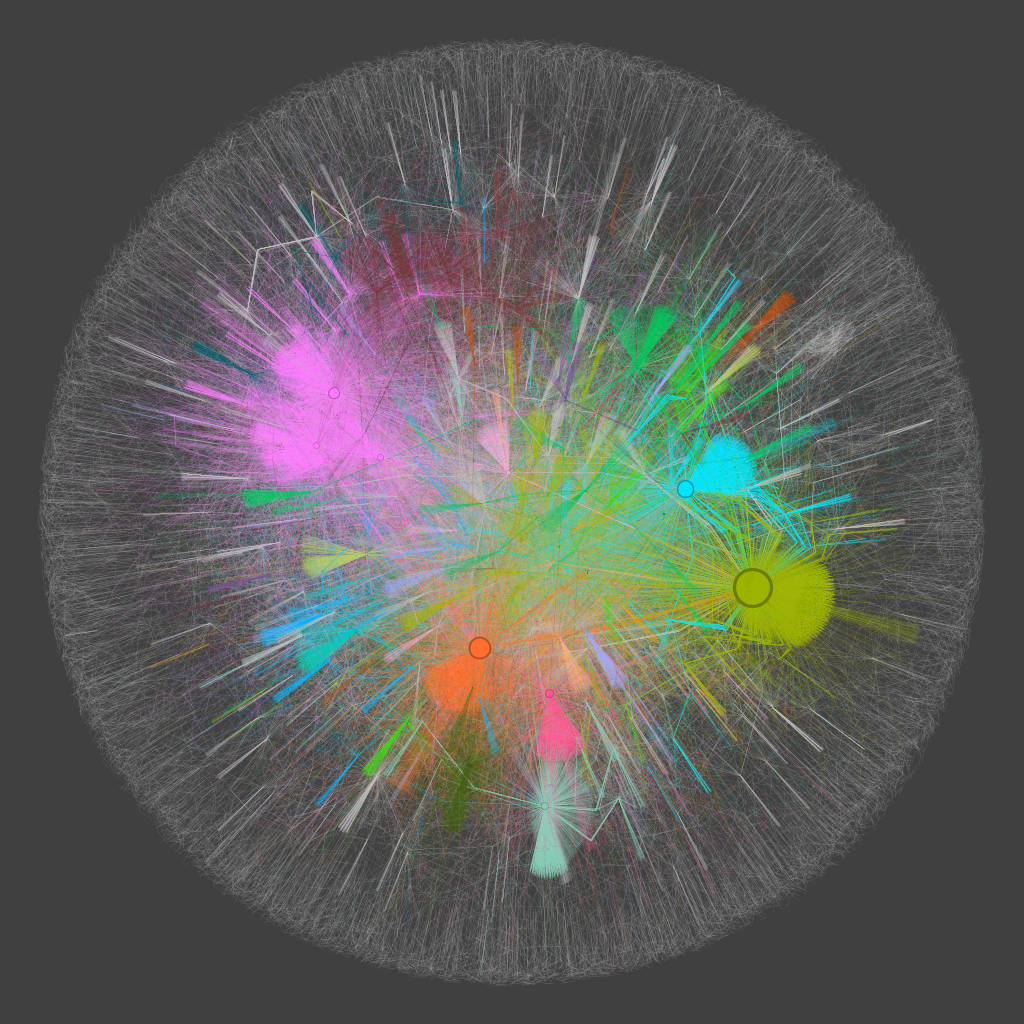
\includegraphics[scale=0.4]{img/A2/Figure.png}
\centering
\caption{Transfers of crypto currency}
\label{fig:Fig}
\end{figure}

In Gephi we can see all connections of the node. If we click on lime green, we can see how it is connected to the most of the nodes.
\begin{figure}[H]
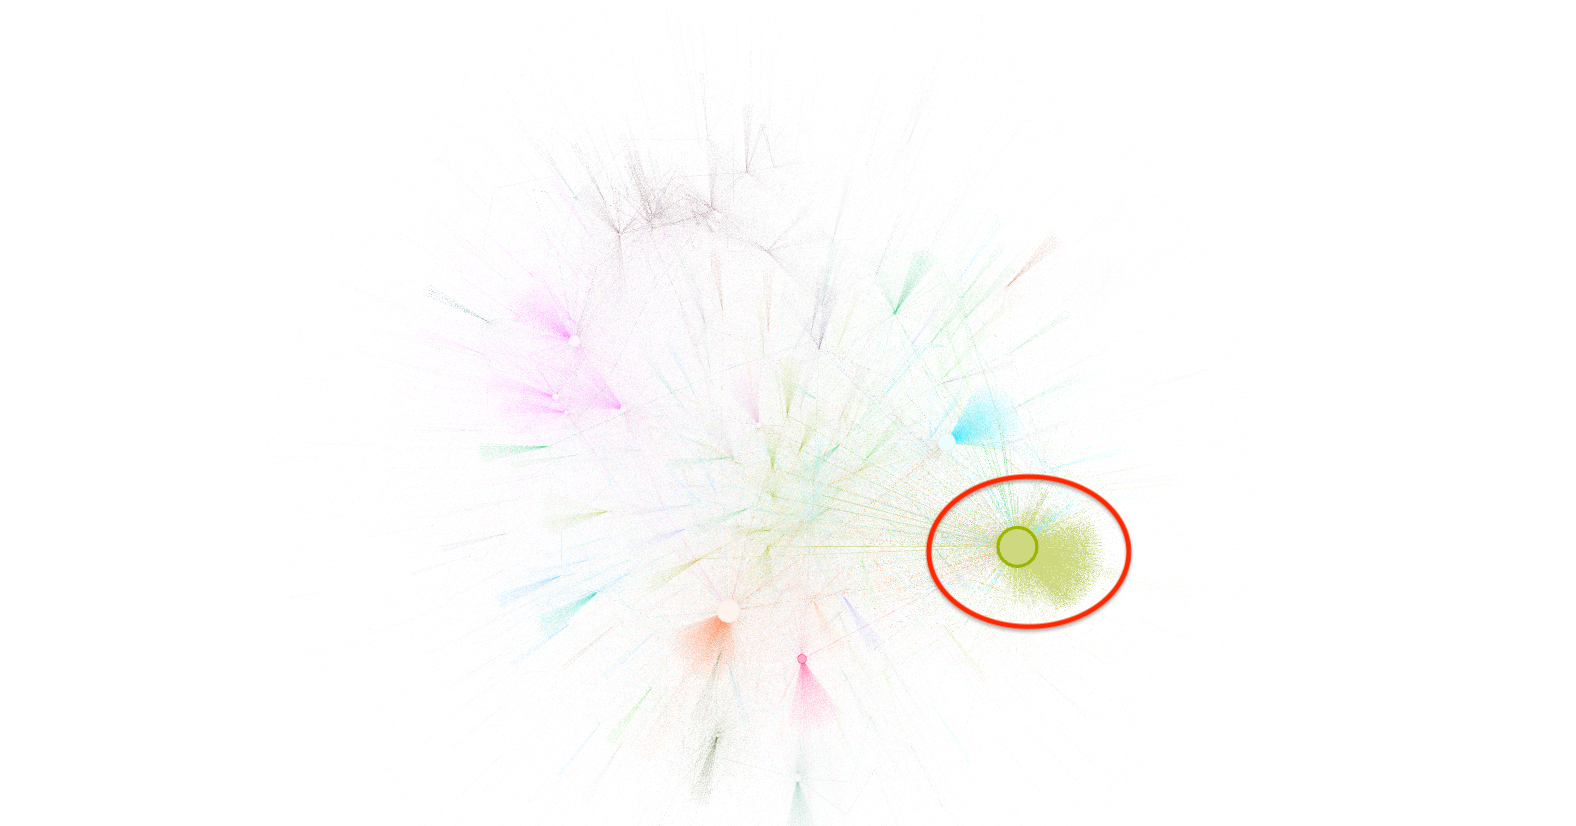
\includegraphics[scale=0.4]{img/A2/Figure1.png}
\centering
\caption{Showcase of biggest node}
\label{fig:Fig1}
\end{figure}

Selecting red (pink) node we can see that number of connections looks similar but less than main node.
\begin{figure}[H]
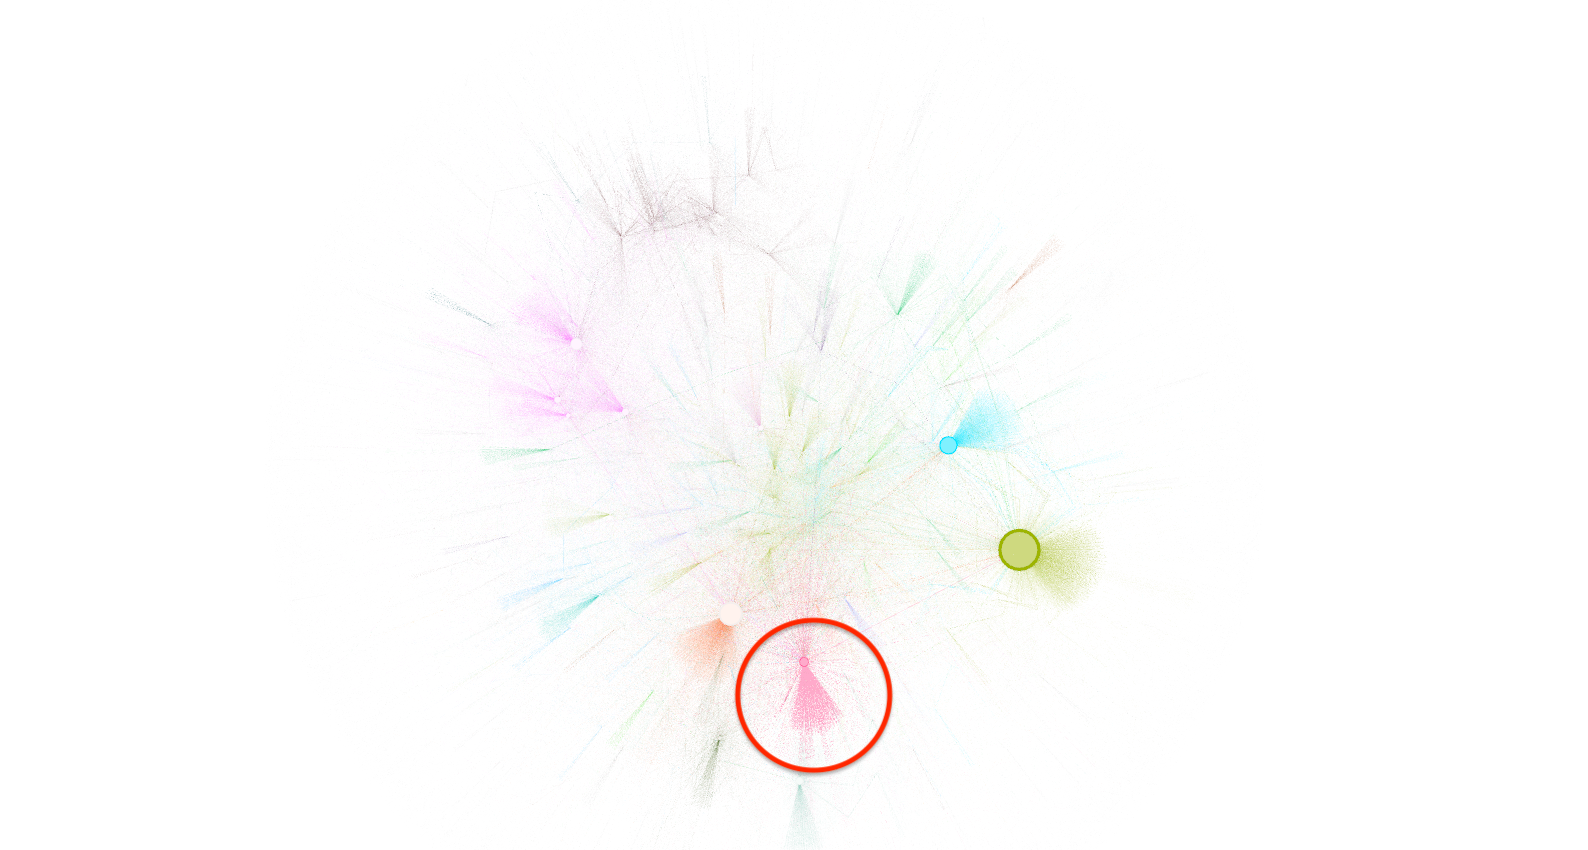
\includegraphics[scale=0.4]{img/A2/Figure2.png}
\centering
\caption{Showcase of smaller node}
\label{fig:Fig2}
\end{figure}

Gephi also generates network (graph) information for us. For example we can see that average degree is 1.177 and modality is 0.82.
\begin{figure}[H]
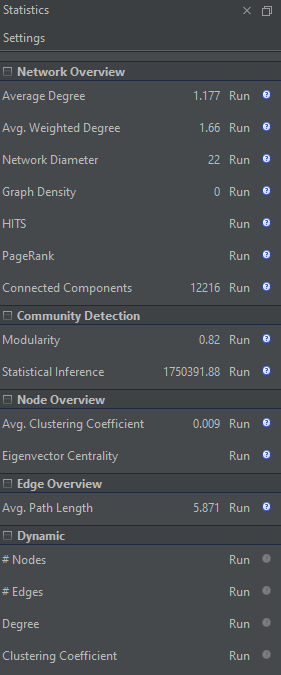
\includegraphics[scale=0.7]{img/A2/Settings1.PNG}
\centering
\caption{Gephi statistics}
\label{fig:Settings1}
\end{figure}

In total, this network has 152165 nodes and 179024 edges.
\begin{figure}[H]
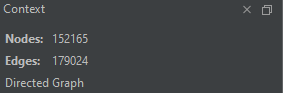
\includegraphics[scale=0.7]{img/A2/Settings2.PNG}
\centering
\caption{List of nodes and edges}
\label{fig:Settings2}
\end{figure}